Negli ultimi anni abbiamo assistito a un'enorme diffusione di Internet e soprattutto di una varietà di dispositivi con i quali è possibile accedervi: mentre agli albori esistevano solamente PC \emph{desktop}, con i quali poter visitare pagine Web per lo più statiche, al giorno d'oggi sono disponibili dispositivi come \emph{smartphone} e \emph{tablet} che ci permettono di rimanere sempre connessi. Grazie al fatto di essere estremamente portatili e semplici da utilizzare, tali dispositivi sono ormai diventati oggetti indispensabili nella vita quotidiana, tanto che oramai la quantità di traffico generata da \emph{smartphone} e \emph{tablet} supera nettamente quella generata dai PC (Figura \ref{fig:traffico-tipologia-dispositivo}). L'incremento della velocità delle connessioni e il progresso tecnologico ha fatto sì che sia possibile consultare qualsiasi tipo di informazione su Internet, dal semplice testo fino a immagini e video.

\begin{figure}[ht]
	\centering
	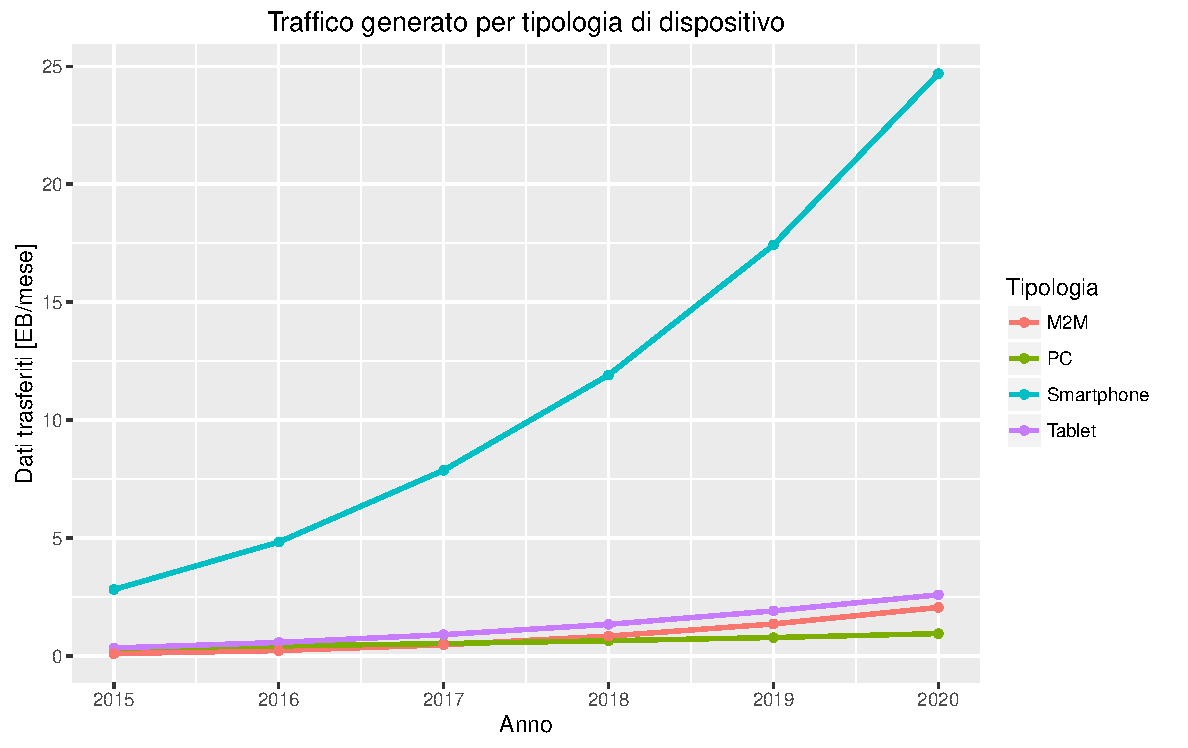
\includegraphics[width=\textwidth]{1-introduzione/Immagini/traffico-dispositivi.pdf}
	\caption[Traffico generato per tipologia di dispositivo]{Traffico generato per tipologia di dispositivo (Fonte: \href{http://www.cisco.com/c/en/us/solutions/collateral/service-provider/visual-networking-index-vni/mobile-white-paper-c11-520862.html}{Cisco}, 2016)\label{fig:traffico-tipologia-dispositivo}}
\end{figure}

Si è persa anche la tradizione che sia un gestore a pubblicare contenuti, in quanto ormai sono direttamente gli utenti a produrre la maggior parte delle informazioni disponibili (Figura \ref{fig:analisi-dati-generati}). Questo fenomeno è stato accentuato con la creazione dei \emph{social network}, che permettono di creare collegamenti tra le persone e dove è possibile condividere qualunque cosa che ognuno trova interessante. Gli utenti vengono così coinvolti nella creazione di contenuti di varia natura, anche di tipo multimediale grazie alla dotazione di fotocamere ad alta risoluzione nei dispositivi.

\begin{figure}[ht]
	\centering
	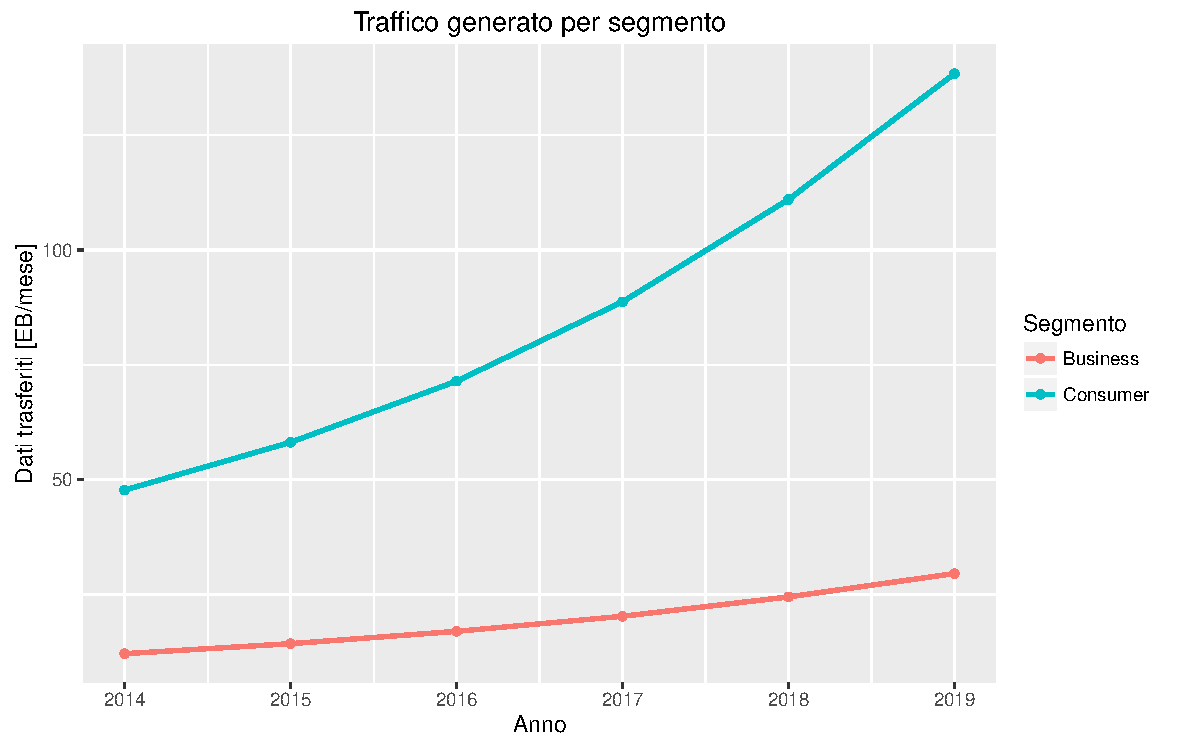
\includegraphics[width=\textwidth]{1-introduzione/Immagini/traffico-consumer-business.pdf}
	\caption[Traffico generato per segmento]{Traffico generato per segmento (Fonte: \href{http://www.cisco.com/c/en/us/solutions/collateral/service-provider/visual-networking-index-vni/VNI_Hyperconnectivity_WP.html}{Cisco}, 2016)\label{fig:analisi-dati-generati}}
\end{figure}

Come si può notare in Figura \ref{fig:traffico-categoria-applicazione} il traffico video e audio è in costante aumento. In particolare il traffico di video sovrasta tutti gli altri, anche a causa della maggior dimensioni di questi contenuti. Questo fenomeno è incentivato dalla diffusione di servizi che permettono lo \emph{streaming} dei contenuti multimediali come YouTube\footnote{YouTube: \url{https://www.youtube.com}} o Netflix\footnote{Netflix: \url{https://www.netflix.com}}.

\begin{figure}[ht]
	\centering
	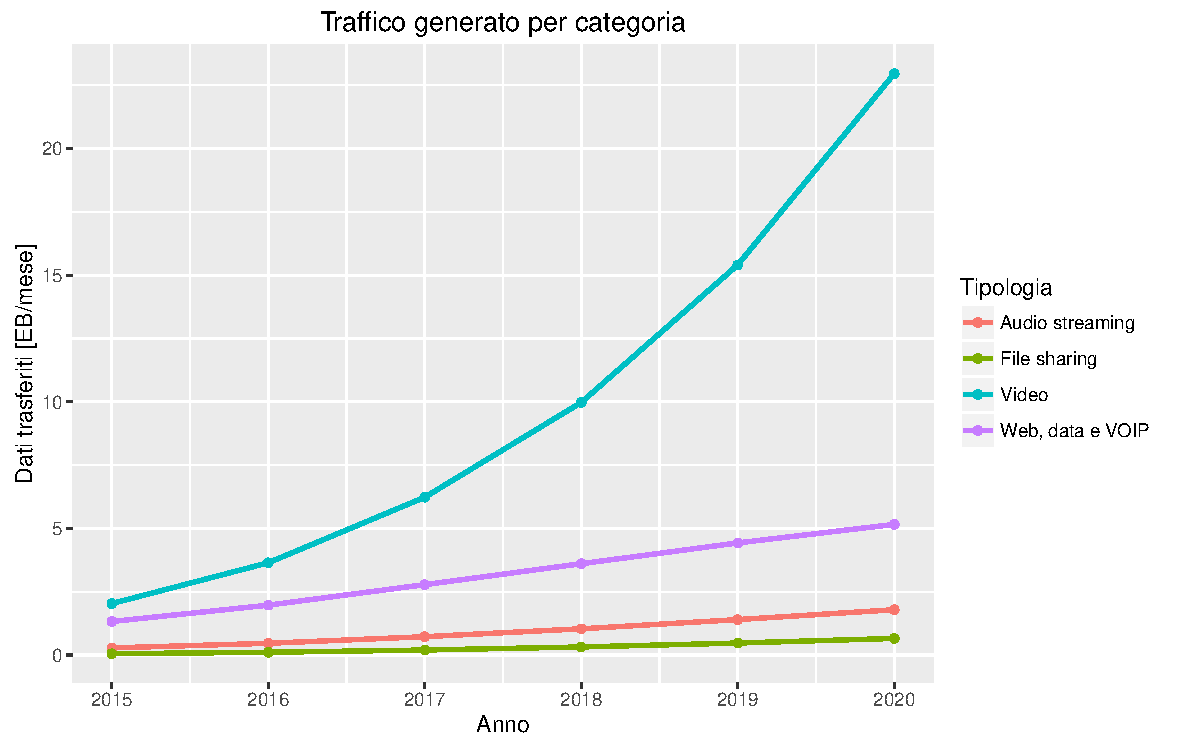
\includegraphics[width=\textwidth]{1-introduzione/Immagini/traffico-categoria.pdf}
	\caption[Traffico generato per categoria]{Traffico generato per categoria (fonte: \href{http://www.cisco.com/c/en/us/solutions/collateral/service-provider/visual-networking-index-vni/mobile-white-paper-c11-520862.html}{Cisco}, 2016)\label{fig:traffico-categoria-applicazione}}
\end{figure}

Internet è quindi diventato una fonte immensa di informazioni, che sono destinate ad aumentare. Questo trend è inoltre accentuato dall'avvento dei dispositivi connessi, cioè l'\emph{Internet of Things}, come è possibile osservare in Figura \ref{fig:traffico-tipologia-dispositivo} nella tipologia \virgolette{M2M} (\emph{Machine to Machine}). L'idea è che qualsiasi dispositivo può essere connesso a Internet per generare informazioni, in particolare tutti quelli provvisti di sensori che possono fornire dati sullo stato dell'ambiente nel quale si trovano.

%Inizio parte del contesto
Uno dei principali problemi che chiunque lavori coi dati vuole cercare di risolvere è ridurre l'\emph{information noise}, migliorando la precisione delle informazioni da mostrare, in maniera che meglio si adattino ai requisiti che caratterizzano le situazioni d'uso.

\upe frequente che le informazioni non vengano acquisite unicamente da una base di dati bensì provengano da più fonti, anche di tipologie diverse tra loro (es.: relazionali, XML, ec..). Basti pensare alla moltitudine di servizi presenti nel Web.

Questo aumento della quantità e dell'eterogeneità delle informazioni, se non propriamente controllato, può provocare un ammasso di dati che genera soltanto confusione piuttosto che fornire elementi utili, riducendo i benefici che invece si potrebbero ricavare da tutte queste informazioni. Tuttavia, distinguere le informazioni rilevanti da quelle che non lo sono è un compito tutt'altro che semplice: alcune informazioni potrebbero essere trattate in maniera differente, anche per lo stesso utente che in diverse situazioni ha bisogno di informazioni differenti. 

Si parla dunque di sistemi \emph{Context-Aware}, che si occupano cioè dell'\emph{acquisizione} del contesto (per esempio tramite l'utilizzo di determinati sensori), l'\emph{astrazione} e il \emph{riconoscimento} del contesto (per esempio per associare un determinato stimolo al contesto) e il \emph{comportamento} adatto alla situazione riconosciuta (per esempio l'esecuzione di un'azione innescata dal contesto) \cite{schmidt2003ubiquitous}. L'utilizzo del \emph{contesto} permette la realizzazione di applicazioni flessibili e personalizzate. 

%Resta aperto il problema di come visualizzare le operazioni e come ricercare le info in modo semplice (Fornire interfaccia per permettere agli utenti di cercare le informazioni)

Una volta acquisite le informazioni nasce tuttavia l'esigenza di definire regole su come mostrarle all'utente finale. Con la diffusione di dispositivi mobili sempre più sofisticati si è resa maggiormente necessaria un'esperienza utente semplice che lo guidi durante le sue attività.

%	parlare di come sia conveniente un meccanismo decori le informazioni testuali con contenuti aggiuntivi, come mappe, foto e altre cose dinamiche}

Per questo motivo ha assunto un ruolo di grande importanza l'esperienza d'uso dell'utente (\emph{User Experience}). Infatti se un'applicazione non è ben strutturata e non è fruibile in modo semplice dall'utente, il numero di utenti che la utilizzeranno calerà sempre di più. Secondo Gary Illyes di Google \virgolette{circa il $ 61\% $ degli utenti che incontrano problemi con siti e \emph{app} su \emph{smartphone} ne abbandonano l'utilizzo volontariamente}\footnote{Search Engine Land Interview to Gary Illyes of Google: \url{http://searchengineland.com/google-may-add-mobile-user-experience-ranking-algorithm-205382}}. Per evitare questo problema è necessario prestare un'attenzione sempre maggiore a come viene progettato tutto il flusso di navigazione e a fornire i dati necessari per poter sfruttare al meglio l'applicazione. L'aggiunta di elementi comprensibili in modo intuitivo come mappe e foto porta l'utente a utilizzare altre aree della mente, come quella della memoria fotografica. In questo modo l'utente può facilmente acquisire conoscenza, utilizzando diversi dati e diverse tipologie di visualizzazione.

%inizio parte di progetto

\upe proprio per cercare nuovi strumenti in grado di migliorare l'esperienza dell'u\-ten\-te nell'esplorazione delle informazioni che nasce il progetto CAMUS. CAMUS (\emph{Context-Aware Mobile mashUpS}) si propone come un \emph{framework} per permettere la realizzazione di \emph{mobile app} che si adattino sia alle preferenze dell'utente sia alla situazione nella quale si trova. L'idea è che l'utilizzo di modelli per definire il contesto e per schematizzare la composizione dell'interfaccia grafica possa portare enormi benefici nell'interazione tra utente e applicazione.
Questo paradigma permette la realizzazione di applicazioni flessibili e personalizzate dove la struttura e i contenuti possono variare in fase di esecuzione in base alle esigenze dell'utente e alla situazione nella quale si trova. Inoltre si vuole sfruttare la multimedialità messa a disposizione dei recenti dispositivi mobili per coinvolgere maggiormente l'utente e semplificare le sue attività.

Dalla sigla è possibile intuire le due anime principali che sono alla base del progetto: i \emph{mashup} e il \emph{contesto}.

Per la tematica dei \emph{mashup} viene preso in considerazione l'aspetto di acquisire le informazioni da più fonti di diverso tipo. CAMUS prevede un sistema flessibile che permette di acquisire informazioni da diverse risorse, andando così ad aumentare la completezza delle informazioni fornite all'utente. Come detto in precedenza, bisogna fare attenzione all'utilizzo di grosse quantità di dati, in quanto se non opportunamente trattate e filtrate possono generare solamente confusione e risultare così poco fruibili dall'utente. Nasce così l'intuizione di utilizzare la modellazione del contesto come metodo per selezionare i servizi che possono fornire i dati più rilevanti per l'utente. Il modello del contesto mette a disposizione lo stato in cui si trova l'utente, le condizioni dell'ambiente che lo circonda e i suoi interessi personali. Queste preziose informazioni possono essere uno strumento determinante per mettere ordine ai dati e fornire così solo le informazioni che sono interessanti.

Nella tesi si andrà ad affrontare la modellazione della situazione nella quale si trova l'utente. \upe un'attività molto delicata, in quanto esistono una moltitudine di parametri che possono definire una particolare situazione. \upe necessario fare una scelta di quali siano gli indicatori più idonei e quali invece possano essere scartati. L'obiettivo è fornire un modello che permetta di definire in maniera adeguata e semplice il contesto, in modo da agevolare l'utente e rispettando i principi di \emph{User Experience} precedentemente citati.

Certamente il problema principale riguarda l'organizzazione fisica delle informazioni. Visto che le applicazioni CAMUS non sono limitate a uno specifico contesto, è necessario prevedere un meccanismo che permetta di adattare la visualizzazione di categorie diverse di informazioni. Come è facilmente intuibile, mostrare un elenco di film è ben diverso da mostrare un elenco di ristoranti. Un primo punto da snodare è quindi relativo alla creazione di uno schema flessibile per la presentazione dei dati che permetta di descrivere come visualizzare queste informazioni sul dispositivo.

Questo schema deve inoltre essere anche in grado di raccogliere informazioni di contorno che permettano di migliorare l'esplorazione di quelle principali. Per esempio, se si sta cercando un ristorante può essere d'aiuto avere a disposizione una galleria di foto del locale con i piatti che offre, una mappa che indichi dove si trova il ristorante o alcune informazioni sul meteo, per decidere se prenotare all'esterno o all'interno. Invece se si sta cercando un film può essere sicuramente d'aiuto avere un trailer da vedere per avere un'idea del film, oppure l'elenco dei cinema che l'hanno in programmazione.

Le operazioni di modellazione descritte sopra non sono alla portata degli utenti, soprattutto per quanto riguarda la modellazione del contesto o la composizione dell'interfaccia grafica. Inoltre, quando il contesto deve descrivere diverse realtà, assume anche dimensioni notevoli. Avere troppe scelte a disposizione rende vani gli sforzi per cercare di mettere ordine nei dati, in quanto verrebbe solamente spostato il problema a un altro livello. L'utente non conosce a fondo la struttura dei dati e non è in grado quindi di comporre al meglio un'interfaccia completa dei servizi ausiliari. La letteratura sui \textit{mashup} propone metodi di sviluppo adatti all'utente finale con poche conoscenze tecniche, in accordo con le discipline dell'\emph{End-User Development} \cite{Cappiello:2015:UAE:2788341.2735632}. Tuttavia, per agevolare l'utente finale in queste situazioni, si è deciso di dare importanza alla figura dell'\emph{esperto di settore}. L'esperto di settore è colui che conosce a fondo l'ambito di utilizzo di una \emph{CAMUS app}. Si ritiene che questa sua conoscenza possa guidare l'utente nelle proprie scelte. Uno dei suoi compiti sarà quello di definire insieme all'utente un profilo, in base alle sue esigenze, in modo che dalla rappresentazione del contesto possano essere eliminate le informazioni non necessarie. Inoltre si occuperà di comporre delle interfacce funzionali sia per la situazione sia per l'utente. In questo modo è possibile avere una varietà di composizioni adatte ai diversi ambiti di utilizzo, alle preferenze dell'utente e ad altri fattori, come la geo-referenziazione.

All'esperto di settore vengono delegati compiti che riguardano maggiormente l'ambito nel quale viene utilizzata l'applicazione. Per questo motivo non è necessario che sia una figura con particolari competenze informatiche. Nel \emph{framework} però saranno necessarie delle fasi più tecniche, per il corretto funzionamento della piattaforma. Queste attività, relative alle configurazioni del sistema, necessitano di competenze soprattutto per quanto riguarda il funzionamento dei servizi. Per questo motivo è necessaria la figura dell'\emph{amministratore}. I suoi compiti sono quelli di creare lo schema globale del contesto, che verrà utilizzato dagli esperti di settore per creare gli schemi personalizzati, e la descrizione dei servizi che il sistema può utilizzare per recuperare le informazioni. L'amministratore può anche dedicarsi all'introduzione nel sistema di nuovi schemi di visualizzazione dei dati utilizzabili nella fase di creazione dell'app finale.

\section{Caso di studio: il turismo\label{sec:caso-studio-turismo}}

In questa sezione introduciamo un caso di studio, che sarà utilizzato nei capitoli seguenti per esemplificare i concetti e le tecniche che saranno illustrate. 

CAMUS ha come obiettivo quello di essere universale, cioè utilizzabile in ambiti anche molto diversi tra loro. Come caso di studio è stato dunque necessario pensare a un ambito che consentisse di sfruttare al meglio le capacità di adattarsi alle varie situazioni nelle quali si può trovare l'utilizzatore dell'\emph{app}.

\upe stato scelto un caso di studio relativo al settore \emph{turistico} proprio per via della sua dinamicità. In particolare si è preso in considerazione il caso di un'agenzia di viaggi che deve proporre ai propri clienti dei pacchetti di viaggio.

L'ambito turistico calza a pennello per gli intenti di CAMUS; un viaggio incomincia dalla sua pianificazione: prima di partire il turista si informa sulla destinazione, su quali hotel sono disponibili, con quali mezzi di trasporto è più conveniente raggiungere la destinazione. In questo frangente, CAMUS si propone come \virgolette{suggeritore} di esperienze di viaggio: permette all'utente di non concentrarsi sul \emph{dove} vuole andare ma sul \emph{cosa} vuole fare. All'utente viene data la possibilità di scegliere l'esperienza di viaggio che vuole intraprendere e proporgli così i pacchetti che corrispondono alle sue scelte.

Le potenzialità di CAMUS non terminano una volta che il viaggiatore sceglie la sua meta: l'\emph{app} gli servirà \emph{durante} il viaggio per informarsi sulle attività da svolgere, le escursioni disponibili, i ristoranti nei quali cenare, ecc. Per esempio, se un utente vuole provare un ristorante tipico della zona, gli basterà aprire l'\emph{app} CAMUS e selezionare che è interessato nella ricerca dei ristoranti che propongono dei menù \emph{tipici} del luogo. Gli verrà quindi mostrato un elenco dei ristoranti che si trovano nei suoi paraggi che rispettano i criteri di ricerca definiti. Inoltre gli verranno fornite indicazioni su come raggiungere il ristorante, sfruttando, se specificato nella richiesta, i mezzi pubblici presenti nella destinazione scelta.

Le due figure principali in questo caso di studio sono quindi: l'\emph{agente di viaggio} e il \emph{turista}. L'\emph{agente} ha il compito di organizzare tutto il viaggio, gestire le prenotazioni, gli spostamenti principali e i soggiorni per il viaggiatore, mentre il \emph{turista} è colui che fisicamente compie il viaggio, che può essere quindi considerato come l'utente finale.

All'agente vengono inoltre demandati i compiti di personalizzazione dell'\emph{app}: questa fase avviene quando il cliente si presenta nell'agenzia di viaggio. A quest'ultimo vengono prima di tutto fatte alcune domande per conoscere il suo profilo, in modo da adattare le scelte che gli verranno mostrate dall'\emph{app}. In questo modo è possibile evitare che al cliente vengano proposte troppe scelte che non siano di suo interesse. Inoltre vengono fissate alcune opzioni che tendono a non cambiare nel corso del viaggio; per esempio se l'utente viaggia con un animale domestico, questa scelta sarà considerata durante tutto il viaggio e l'utente non dovrà specificarla per ogni nuova ricerca di informazioni. %\footnote{CAMUS si schiera contro l'abbandono degli animali: \url{http://www.emergenza24.org/salvaunamico/}}

L'ulteriore compito che può svolgere l'agente è quello di personalizzare l'aspetto grafico dell'\emph{app} qualora ritenga che sia necessario. Con CAMUS vengono proposti alcuni \emph{template} predefiniti per ogni categoria di informazioni e viene lasciata libera scelta all'agente se utilizzarli così come sono o modificarli. Per esempio può decidere che alcuni elementi del \emph{template} siano rimossi o aggiungerne tra quelli disponibili all'interno dell'applicazione, a seconda della disponibilità dei termini presenti nella categoria di informazioni, oppure può modificare lo stile dell'elemento grafico.

Come si può notare da questo breve esempio, l'utilizzo di CAMUS in un'agenzia viaggi permette di fornire un servizio più coinvolgente ai propri clienti. La realizzazione di \emph{app} personalizzate permette al turista di effettuare scelte migliori e di proprio interesse. Inoltre estende la capacità dell'agenzia di fornire un'assistenza al proprio cliente anche durante il viaggio: si può affermare che un'\emph{app} CAMUS assume il ruolo di \emph{assistente di viaggio} e guida il turista durante tutte le fasi della sua esperienza di viaggio.

\section{Struttura della tesi}

Viene ora fornita una panoramica sulla struttura di questa tesi:

\begin{itemize}
	\item 
	Nel Capitolo \ref{ch:nozioni-preliminari}, dopo aver introdotto i modelli che saranno utilizzati nel resto della tesi, si discute la letteratura sull'argomento e le tecnologie impiegate per lo sviluppo del prototipo
	\item 
	Nel Capitolo \ref{ch:metodologia-camus} si entra nei dettagli del progetto CAMUS andando a fornire un contesto più ampio di quello appena descritto e mettendo in risalto gli obiettivi che si vogliono raggiungere. In seguito saranno analizzate nel dettaglio le logiche alla base del \emph{framework}
	\item 
	Nel Capitolo \ref{ch:progettazione-alto-livello} viene introdotta l'architettura della piattaforma. Verrà inoltre fornito uno schema del flusso di esecuzione delle attività ed esposto un caso d'uso reale per chiarire meglio la sequenza delle attività
	\item 
	Nei Capitoli \ref{ch:implementazione-backend} e \ref{ch:implementazione-app} viene analizzata nel dettaglio l'implementazione rispettivamente lato \emph{backend} e \emph{mobile app}. Si analizzano i componenti che formano il sistema e le scelte tecnologiche che hanno portato alla realizzazione del prototipo
	\item 
	Nel Capitolo \ref{ch:performance} si analizzano le prestazioni della soluzione implementata, simulando alcuni casi d'uso simili alle condizioni di regime della piattaforma
	\item 
	Nel Capitolo \ref{ch:conclusioni} si discuteranno le conclusioni del lavoro relative al progetto e alcuni spunti per futuri miglioramenti al \emph{framework}
\end{itemize}